% Copyright (C) 2023  Andrea Patrizi (AndrePatri, andreapatrizi1b6e6@gmail.com)
% 
% This file is part of PhDBiorobBeamerTemplate and distributed under the General Public License version 2 license.
% 
% PhDBiorobBeamerTemplate is free software: you can redistribute it and/or modify
% it under the terms of the GNU General Public License as published by
% the Free Software Foundation, either version 2 of the License, or
% (at your option) any later version.
% 
% PhDBiorobBeamerTemplate is distributed in the hope that it will be useful,
% but WITHOUT ANY WARRANTY; without even the implied warranty of
% MERCHANTABILITY or FITNESS FOR A PARTICULAR PURPOSE.  See the
% GNU General Public License for more details.
% 
% You should have received a copy of the GNU General Public License
% along with PhDBiorobBeamerTemplate.  If not, see <http://www.gnu.org/licenses/>.
% 
\begin{frame}{Example slide with conceptual boxes}

\begin{columns}[c, onlytextwidth]
	    	
	    	\column{0.8\textwidth}
	    	\onslide<1->{
	    	\custombox{left}{0.98\textwidth}{white}{\textbf{Belief}: {I believe robotics is beautiful.}}
	    	}
%	    	\\
	    	\onslide<2->{
	    	\custombox{left}{0.98\textwidth}{white}{\textbf{Goal}: {Disseminate knowledge}}
   			}
   			
   			\onslide<3->{
   			\custombox{left}{0.98\textwidth}{white}{\textbf{Proposed approach}: {Distribute this awesome template}}
   			}
%   			
    		\onslide<4->{
    		\column{0.2\textwidth}
    		\begin{figure}[h]
    			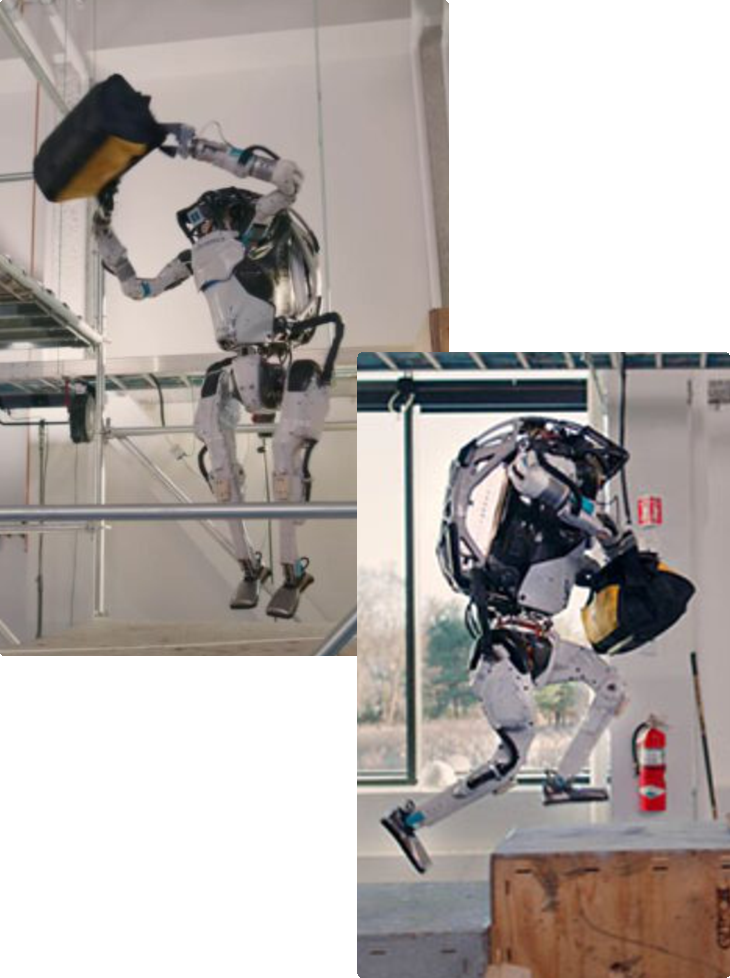
\includegraphics[scale=0.25,keepaspectratio]{docs/imgs/atlas.pdf}
    			\caption*{Boston Dynamics' Atlas showing impressive human-like loco-manipulation skills.}
    		\end{figure}
    		}
    		
\end{columns}

\end{frame}